\PassOptionsToPackage{unicode=true}{hyperref} % options for packages loaded elsewhere
\PassOptionsToPackage{hyphens}{url}
%
\documentclass[ignorenonframetext,]{beamer}
\usepackage{pgfpages}
\setbeamertemplate{caption}[numbered]
\setbeamertemplate{caption label separator}{: }
\setbeamercolor{caption name}{fg=normal text.fg}
\beamertemplatenavigationsymbolsempty
\usepackage{lmodern}
\usepackage{amssymb,amsmath}
\usepackage{ifxetex,ifluatex}
\usepackage{fixltx2e} % provides \textsubscript
\ifnum 0\ifxetex 1\fi\ifluatex 1\fi=0 % if pdftex
  \usepackage[T1]{fontenc}
  \usepackage[utf8]{inputenc}
  \usepackage{textcomp} % provides euro and other symbols
\else % if luatex or xelatex
  \usepackage{unicode-math}
  \defaultfontfeatures{Ligatures=TeX,Scale=MatchLowercase}
\fi
% use upquote if available, for straight quotes in verbatim environments
\IfFileExists{upquote.sty}{\usepackage{upquote}}{}
% use microtype if available
\IfFileExists{microtype.sty}{%
\usepackage[]{microtype}
\UseMicrotypeSet[protrusion]{basicmath} % disable protrusion for tt fonts
}{}
\IfFileExists{parskip.sty}{%
\usepackage{parskip}
}{% else
\setlength{\parindent}{0pt}
\setlength{\parskip}{6pt plus 2pt minus 1pt}
}
\usepackage{hyperref}
\hypersetup{
            pdftitle={Crash Introduction to markovchain R package},
            pdfauthor={Giorgio Alfredo Spedicato, Ph.D C.Stat ACAS},
            pdfborder={0 0 0},
            breaklinks=true}
\urlstyle{same}  % don't use monospace font for urls
\newif\ifbibliography
\usepackage{color}
\usepackage{fancyvrb}
\newcommand{\VerbBar}{|}
\newcommand{\VERB}{\Verb[commandchars=\\\{\}]}
\DefineVerbatimEnvironment{Highlighting}{Verbatim}{commandchars=\\\{\}}
% Add ',fontsize=\small' for more characters per line
\usepackage{framed}
\definecolor{shadecolor}{RGB}{248,248,248}
\newenvironment{Shaded}{\begin{snugshade}}{\end{snugshade}}
\newcommand{\AlertTok}[1]{\textcolor[rgb]{0.94,0.16,0.16}{#1}}
\newcommand{\AnnotationTok}[1]{\textcolor[rgb]{0.56,0.35,0.01}{\textbf{\textit{#1}}}}
\newcommand{\AttributeTok}[1]{\textcolor[rgb]{0.77,0.63,0.00}{#1}}
\newcommand{\BaseNTok}[1]{\textcolor[rgb]{0.00,0.00,0.81}{#1}}
\newcommand{\BuiltInTok}[1]{#1}
\newcommand{\CharTok}[1]{\textcolor[rgb]{0.31,0.60,0.02}{#1}}
\newcommand{\CommentTok}[1]{\textcolor[rgb]{0.56,0.35,0.01}{\textit{#1}}}
\newcommand{\CommentVarTok}[1]{\textcolor[rgb]{0.56,0.35,0.01}{\textbf{\textit{#1}}}}
\newcommand{\ConstantTok}[1]{\textcolor[rgb]{0.00,0.00,0.00}{#1}}
\newcommand{\ControlFlowTok}[1]{\textcolor[rgb]{0.13,0.29,0.53}{\textbf{#1}}}
\newcommand{\DataTypeTok}[1]{\textcolor[rgb]{0.13,0.29,0.53}{#1}}
\newcommand{\DecValTok}[1]{\textcolor[rgb]{0.00,0.00,0.81}{#1}}
\newcommand{\DocumentationTok}[1]{\textcolor[rgb]{0.56,0.35,0.01}{\textbf{\textit{#1}}}}
\newcommand{\ErrorTok}[1]{\textcolor[rgb]{0.64,0.00,0.00}{\textbf{#1}}}
\newcommand{\ExtensionTok}[1]{#1}
\newcommand{\FloatTok}[1]{\textcolor[rgb]{0.00,0.00,0.81}{#1}}
\newcommand{\FunctionTok}[1]{\textcolor[rgb]{0.00,0.00,0.00}{#1}}
\newcommand{\ImportTok}[1]{#1}
\newcommand{\InformationTok}[1]{\textcolor[rgb]{0.56,0.35,0.01}{\textbf{\textit{#1}}}}
\newcommand{\KeywordTok}[1]{\textcolor[rgb]{0.13,0.29,0.53}{\textbf{#1}}}
\newcommand{\NormalTok}[1]{#1}
\newcommand{\OperatorTok}[1]{\textcolor[rgb]{0.81,0.36,0.00}{\textbf{#1}}}
\newcommand{\OtherTok}[1]{\textcolor[rgb]{0.56,0.35,0.01}{#1}}
\newcommand{\PreprocessorTok}[1]{\textcolor[rgb]{0.56,0.35,0.01}{\textit{#1}}}
\newcommand{\RegionMarkerTok}[1]{#1}
\newcommand{\SpecialCharTok}[1]{\textcolor[rgb]{0.00,0.00,0.00}{#1}}
\newcommand{\SpecialStringTok}[1]{\textcolor[rgb]{0.31,0.60,0.02}{#1}}
\newcommand{\StringTok}[1]{\textcolor[rgb]{0.31,0.60,0.02}{#1}}
\newcommand{\VariableTok}[1]{\textcolor[rgb]{0.00,0.00,0.00}{#1}}
\newcommand{\VerbatimStringTok}[1]{\textcolor[rgb]{0.31,0.60,0.02}{#1}}
\newcommand{\WarningTok}[1]{\textcolor[rgb]{0.56,0.35,0.01}{\textbf{\textit{#1}}}}
\usepackage{graphicx,grffile}
\makeatletter
\def\maxwidth{\ifdim\Gin@nat@width>\linewidth\linewidth\else\Gin@nat@width\fi}
\def\maxheight{\ifdim\Gin@nat@height>\textheight\textheight\else\Gin@nat@height\fi}
\makeatother
% Scale images if necessary, so that they will not overflow the page
% margins by default, and it is still possible to overwrite the defaults
% using explicit options in \includegraphics[width, height, ...]{}
\setkeys{Gin}{width=\maxwidth,height=\maxheight,keepaspectratio}
% Prevent slide breaks in the middle of a paragraph:
\widowpenalties 1 10000
\raggedbottom
\setbeamertemplate{part page}{
\centering
\begin{beamercolorbox}[sep=16pt,center]{part title}
  \usebeamerfont{part title}\insertpart\par
\end{beamercolorbox}
}
\setbeamertemplate{section page}{
\centering
\begin{beamercolorbox}[sep=12pt,center]{part title}
  \usebeamerfont{section title}\insertsection\par
\end{beamercolorbox}
}
\setbeamertemplate{subsection page}{
\centering
\begin{beamercolorbox}[sep=8pt,center]{part title}
  \usebeamerfont{subsection title}\insertsubsection\par
\end{beamercolorbox}
}
\AtBeginPart{
  \frame{\partpage}
}
\AtBeginSection{
  \ifbibliography
  \else
    \frame{\sectionpage}
  \fi
}
\AtBeginSubsection{
  \frame{\subsectionpage}
}
\setlength{\emergencystretch}{3em}  % prevent overfull lines
\providecommand{\tightlist}{%
  \setlength{\itemsep}{0pt}\setlength{\parskip}{0pt}}
\setcounter{secnumdepth}{0}

% set default figure placement to htbp
\makeatletter
\def\fps@figure{htbp}
\makeatother

\usepackage{url}
\providecommand{\tightlist}{
  \setlength{\itemsep}{0pt}\setlength{\parskip}{0pt}
}

\title{Crash Introduction to markovchain R package}
\author{Giorgio Alfredo Spedicato, Ph.D C.Stat ACAS}
\date{2019-09-13}

\begin{document}
\frame{\titlepage}

\begin{frame}
\tableofcontents[hideallsubsections]
\end{frame}
\begin{frame}

\end{frame}

\begin{frame}{Intro}
\protect\hypertarget{intro}{}

\begin{itemize}
\tightlist
\item
  The markovchain package (Spedicato 2017) will be introduced.
\item
  The package is intended to provide S4 classes to perform probabilistic
  and statistical analysis of Discrete Time Markov Chains (DTMC). See
  (Brémaud 1999) for a theoretical review of the mathematics underlying
  the DTMC models.
\item
  The vignette will show: how to load the package and create a DTMC, how
  to manage a DTMC, how to perform basic probabilistic analysis, how to
  fit a DTMC.
\end{itemize}

\end{frame}

\begin{frame}

\begin{itemize}
\tightlist
\item
  The package is on Cran since Summer 2013.
\item
  It requires a recent version of R (\textgreater{}=3.0). Since version
  0.2 parts of code have been moved to Rcpp (Eddelbuettel 2013).
\item
  The package won a slot in Google Summer of Code 2015 for optimizing
  internals and expanding functionalities.
\end{itemize}

\end{frame}

\begin{frame}[fragile]{First moves into the markovchain package}
\protect\hypertarget{first-moves-into-the-markovchain-package}{}

\begin{block}{Loading the package}

\begin{itemize}
\tightlist
\item
  The package is loaded using
\end{itemize}

\begin{Shaded}
\begin{Highlighting}[]
\CommentTok{#load the package}
\KeywordTok{library}\NormalTok{(markovchain) }
\end{Highlighting}
\end{Shaded}

\begin{verbatim}
## Package:  markovchain
## Version:  0.8.0
## Date:     2019-09-13
## BugReport: http://github.com/spedygiorgio/markovchain/issues
\end{verbatim}

\end{block}

\end{frame}

\begin{frame}[fragile]

\begin{block}{Creating a DTMC}

\begin{itemize}
\tightlist
\item
  DTMC can be easily create following standard S4 classes syntax. The
  show method displays it.
\end{itemize}

\begin{Shaded}
\begin{Highlighting}[]
\NormalTok{tmA <-}\StringTok{ }\KeywordTok{matrix}\NormalTok{(}\KeywordTok{c}\NormalTok{(}\DecValTok{0}\NormalTok{,}\FloatTok{0.5}\NormalTok{,}\FloatTok{0.5}\NormalTok{,.}\DecValTok{5}\NormalTok{,}\DecValTok{0}\NormalTok{,.}\DecValTok{5}\NormalTok{,.}\DecValTok{5}\NormalTok{,.}\DecValTok{5}\NormalTok{,}\DecValTok{0}\NormalTok{),}\DataTypeTok{nrow =} \DecValTok{3}\NormalTok{,}
              \DataTypeTok{byrow =} \OtherTok{TRUE}\NormalTok{) }\CommentTok{#define the transition matrix}
\NormalTok{dtmcA <-}\StringTok{ }\KeywordTok{new}\NormalTok{(}\StringTok{"markovchain"}\NormalTok{,}\DataTypeTok{transitionMatrix=}\NormalTok{tmA, }
             \DataTypeTok{states=}\KeywordTok{c}\NormalTok{(}\StringTok{"a"}\NormalTok{,}\StringTok{"b"}\NormalTok{,}\StringTok{"c"}\NormalTok{), }
             \DataTypeTok{name=}\StringTok{"MarkovChain A"}\NormalTok{) }\CommentTok{#create the DTMC}
\NormalTok{dtmcA}
\end{Highlighting}
\end{Shaded}

\begin{verbatim}
## MarkovChain A 
##  A  3 - dimensional discrete Markov Chain defined by the following states: 
##  a, b, c 
##  The transition matrix  (by rows)  is defined as follows: 
##     a   b   c
## a 0.0 0.5 0.5
## b 0.5 0.0 0.5
## c 0.5 0.5 0.0
\end{verbatim}

\end{block}

\end{frame}

\begin{frame}[fragile]

\begin{itemize}
\tightlist
\item
  Otherwise, it can also be created directly coercing a matrix.
\end{itemize}

\begin{Shaded}
\begin{Highlighting}[]
\NormalTok{dtmcA2<-}\KeywordTok{as}\NormalTok{(tmA, }\StringTok{"markovchain"}\NormalTok{) }\CommentTok{#using coerce from matrix}
\KeywordTok{states}\NormalTok{(dtmcA2) }\CommentTok{#note default names assigned to states}
\end{Highlighting}
\end{Shaded}

\begin{verbatim}
## [1] "s1" "s2" "s3"
\end{verbatim}

\end{frame}

\begin{frame}[fragile]

\begin{itemize}
\tightlist
\item
  It is also possible to display a DTMC, using igraph package (Csardi
  and Nepusz 2006) capabilities
\end{itemize}

\begin{Shaded}
\begin{Highlighting}[]
\KeywordTok{plot}\NormalTok{(dtmcA)}
\end{Highlighting}
\end{Shaded}

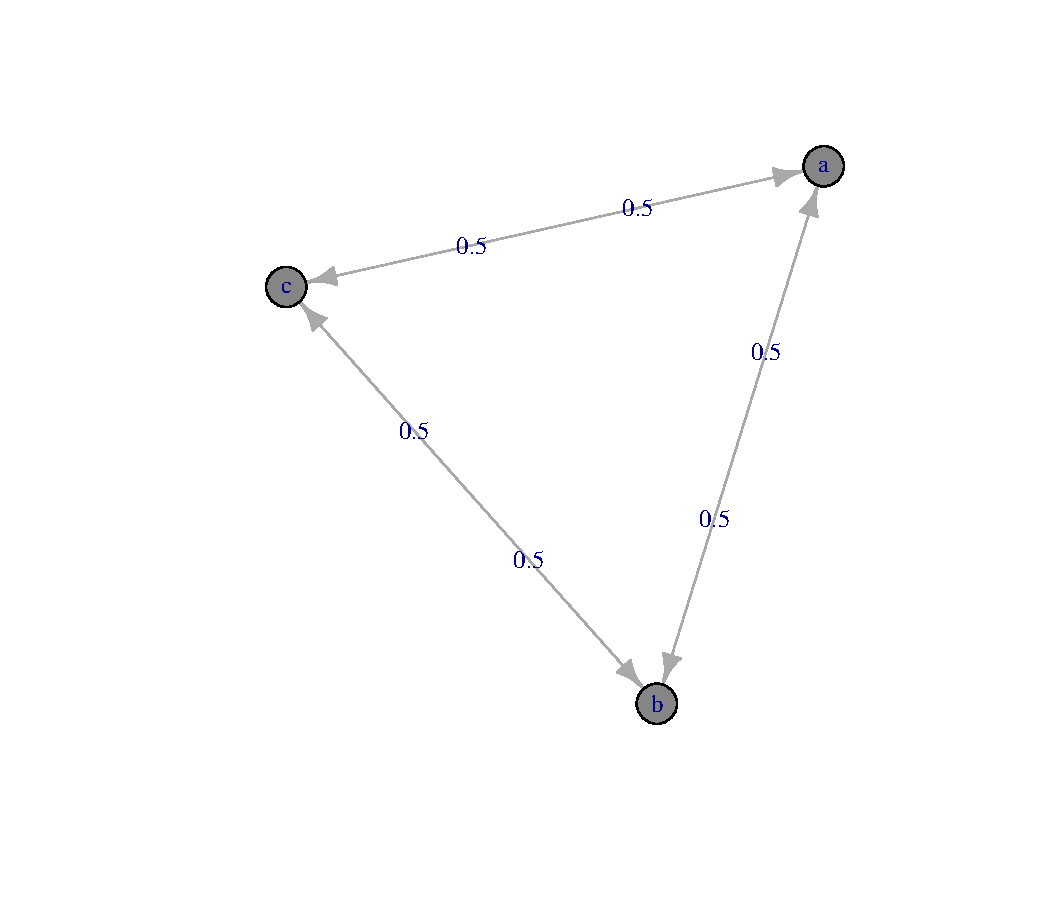
\includegraphics{/tmp/RtmpHzhVBQ/file34611c37d21a/articles/markvochain_crash_intro_files/figure-beamer/plot-1.pdf}

\end{frame}

\begin{frame}[fragile]{Probabilistic analysis}
\protect\hypertarget{probabilistic-analysis}{}

\begin{block}{The basic}

\begin{itemize}
\tightlist
\item
  It is possible to access transition probabilities and to perform basic
  operations.
\item
  Similarly, it is possible to access the conditional distribution of
  states, \(Pr\left ( X_{t+1} | X_{t}=s \right )\)
\end{itemize}

\begin{Shaded}
\begin{Highlighting}[]
\NormalTok{dtmcA[}\DecValTok{2}\NormalTok{,}\DecValTok{3}\NormalTok{] }\CommentTok{#using [ method}
\end{Highlighting}
\end{Shaded}

\begin{verbatim}
## [1] 0.5
\end{verbatim}

\begin{Shaded}
\begin{Highlighting}[]
\KeywordTok{transitionProbability}\NormalTok{(dtmcA, }
                      \StringTok{"b"}\NormalTok{,}\StringTok{"c"}\NormalTok{) }\CommentTok{#using specific S4 method}
\end{Highlighting}
\end{Shaded}

\begin{verbatim}
## [1] 0.5
\end{verbatim}

\begin{Shaded}
\begin{Highlighting}[]
\KeywordTok{conditionalDistribution}\NormalTok{(dtmcA,}\StringTok{"b"}\NormalTok{)}
\end{Highlighting}
\end{Shaded}

\begin{verbatim}
##   a   b   c 
## 0.5 0.0 0.5
\end{verbatim}

\end{block}

\end{frame}

\begin{frame}[fragile]

\begin{itemize}
\tightlist
\item
  It is possible to simulate states distribution after n-steps
\end{itemize}

\begin{Shaded}
\begin{Highlighting}[]
\NormalTok{initialState<-}\KeywordTok{c}\NormalTok{(}\DecValTok{0}\NormalTok{,}\DecValTok{1}\NormalTok{,}\DecValTok{0}\NormalTok{)}
\NormalTok{steps<-}\DecValTok{4}
\NormalTok{finalState<-initialState}\OperatorTok{*}\NormalTok{dtmcA}\OperatorTok{^}\NormalTok{steps }\CommentTok{#using power operator}
\NormalTok{finalState}
\end{Highlighting}
\end{Shaded}

\begin{verbatim}
##           a     b      c
## [1,] 0.3125 0.375 0.3125
\end{verbatim}

\end{frame}

\begin{frame}[fragile]

\begin{itemize}
\tightlist
\item
  As well as steady states distribution
\end{itemize}

\begin{Shaded}
\begin{Highlighting}[]
\KeywordTok{steadyStates}\NormalTok{(dtmcA) }\CommentTok{#S4 method}
\end{Highlighting}
\end{Shaded}

\begin{verbatim}
##              a         b         c
## [1,] 0.3333333 0.3333333 0.3333333
\end{verbatim}

\end{frame}

\begin{frame}[fragile]

\begin{block}{Advanced}

\begin{itemize}
\tightlist
\item
  We use an example found on Mathematica Web page, (Wolfram Research
  2013)
\end{itemize}

\begin{Shaded}
\begin{Highlighting}[]
\NormalTok{E <-}\StringTok{ }\KeywordTok{matrix}\NormalTok{(}\DecValTok{0}\NormalTok{, }\DataTypeTok{nrow =} \DecValTok{4}\NormalTok{, }\DataTypeTok{ncol =} \DecValTok{4}\NormalTok{)}
\NormalTok{E[}\DecValTok{1}\NormalTok{, }\DecValTok{2}\NormalTok{] <-}\StringTok{ }\DecValTok{1}\NormalTok{;E[}\DecValTok{2}\NormalTok{, }\DecValTok{1}\NormalTok{] <-}\StringTok{ }\DecValTok{1}\OperatorTok{/}\DecValTok{3}\NormalTok{; E[}\DecValTok{2}\NormalTok{, }\DecValTok{3}\NormalTok{] <-}\StringTok{ }\DecValTok{2}\OperatorTok{/}\DecValTok{3}
\NormalTok{E[}\DecValTok{3}\NormalTok{,}\DecValTok{2}\NormalTok{] <-}\StringTok{ }\DecValTok{1}\OperatorTok{/}\DecValTok{4}\NormalTok{; E[}\DecValTok{3}\NormalTok{, }\DecValTok{4}\NormalTok{] <-}\StringTok{ }\DecValTok{3}\OperatorTok{/}\DecValTok{4}\NormalTok{; E[}\DecValTok{4}\NormalTok{, }\DecValTok{3}\NormalTok{] <-}\StringTok{ }\DecValTok{1}
\NormalTok{mcMathematica <-}\StringTok{ }\KeywordTok{new}\NormalTok{(}\StringTok{"markovchain"}\NormalTok{, }\DataTypeTok{states =} \KeywordTok{c}\NormalTok{(}\StringTok{"a"}\NormalTok{, }\StringTok{"b"}\NormalTok{, }\StringTok{"c"}\NormalTok{, }\StringTok{"d"}\NormalTok{),}
                     \DataTypeTok{transitionMatrix =}\NormalTok{ E,}\DataTypeTok{name =} \StringTok{"Mathematica"}\NormalTok{)}
\end{Highlighting}
\end{Shaded}

\end{block}

\end{frame}

\begin{frame}[fragile]

\begin{itemize}
\tightlist
\item
  The summary method shows the proprieties of the DTCM
\end{itemize}

\begin{Shaded}
\begin{Highlighting}[]
\KeywordTok{summary}\NormalTok{(mcMathematica)}
\end{Highlighting}
\end{Shaded}

\begin{verbatim}
## Mathematica  Markov chain that is composed by: 
## Closed classes: 
## a b c d 
## Recurrent classes: 
## {a,b,c,d}
## Transient classes: 
## NONE 
## The Markov chain is irreducible 
## The absorbing states are: NONE
\end{verbatim}

\end{frame}

\begin{frame}{Estimation and simulation}
\protect\hypertarget{estimation-and-simulation}{}

The package permits to fit a DTMC estimating the transition matrix from
a sequence of data. - createSequenceMatrix returns a function showing
previous vs actual states from the pairs in a given sequence.

\end{frame}

\begin{frame}[fragile]

\begin{Shaded}
\begin{Highlighting}[]
\CommentTok{#using Alofi rainfall dataset}
\KeywordTok{data}\NormalTok{(rain) }
\NormalTok{mysequence<-rain}\OperatorTok{$}\NormalTok{rain}
\KeywordTok{createSequenceMatrix}\NormalTok{(mysequence)}
\end{Highlighting}
\end{Shaded}

\begin{verbatim}
##       0 1-5  6+
## 0   362 126  60
## 1-5 136  90  68
## 6+   50  79 124
\end{verbatim}

\end{frame}

\begin{frame}[fragile]

\begin{itemize}
\tightlist
\item
  markovchainFit function allows to obtain the estimated transition
  matric and the confidence levels (using elliptic MLE hyphotesis).
\end{itemize}

\begin{Shaded}
\begin{Highlighting}[]
\NormalTok{myFit<-}\KeywordTok{markovchainFit}\NormalTok{(}\DataTypeTok{data=}\NormalTok{mysequence,}\DataTypeTok{confidencelevel =} \FloatTok{.9}\NormalTok{,}\DataTypeTok{method =} \StringTok{"mle"}\NormalTok{)}
\NormalTok{myFit}
\end{Highlighting}
\end{Shaded}

\begin{verbatim}
## $estimate
## MLE Fit 
##  A  3 - dimensional discrete Markov Chain defined by the following states: 
##  0, 1-5, 6+ 
##  The transition matrix  (by rows)  is defined as follows: 
##             0       1-5        6+
## 0   0.6605839 0.2299270 0.1094891
## 1-5 0.4625850 0.3061224 0.2312925
## 6+  0.1976285 0.3122530 0.4901186
## 
## 
## $standardError
##              0        1-5         6+
## 0   0.03471952 0.02048353 0.01413498
## 1-5 0.03966634 0.03226814 0.02804834
## 6+  0.02794888 0.03513120 0.04401395
## 
## $confidenceLevel
## [1] 0.9
## 
## $lowerEndpointMatrix
##             0       1-5         6+
## 0   0.6034754 0.1962346 0.08623909
## 1-5 0.3973397 0.2530461 0.18515711
## 6+  0.1516566 0.2544673 0.41772208
## 
## $upperEndpointMatrix
##             0       1-5        6+
## 0   0.7176925 0.2636194 0.1327390
## 1-5 0.5278304 0.3591988 0.2774279
## 6+  0.2436003 0.3700386 0.5625151
## 
## $logLikelihood
## [1] -1040.419
\end{verbatim}

\end{frame}

\begin{frame}[fragile]

\begin{itemize}
\tightlist
\item
  See the vignettes for further fitting methods as well as for
  functionalities targeted on non - homogeneous Markov chains.
\end{itemize}

\begin{Shaded}
\begin{Highlighting}[]
\NormalTok{alofiMc<-myFit}\OperatorTok{$}\NormalTok{estimate}
\NormalTok{alofiMc}
\end{Highlighting}
\end{Shaded}

\begin{verbatim}
## MLE Fit 
##  A  3 - dimensional discrete Markov Chain defined by the following states: 
##  0, 1-5, 6+ 
##  The transition matrix  (by rows)  is defined as follows: 
##             0       1-5        6+
## 0   0.6605839 0.2299270 0.1094891
## 1-5 0.4625850 0.3061224 0.2312925
## 6+  0.1976285 0.3122530 0.4901186
\end{verbatim}

\end{frame}

\begin{frame}[allowframebreaks]{Bibliography}
\protect\hypertarget{bibliography}{}

\hypertarget{refs}{}
\leavevmode\hypertarget{ref-bremaud1999discrete}{}%
Brémaud, Pierre. 1999. ``Discrete-Time Markov Models.'' In \emph{Markov
Chains}, 53--93. Springer.

\leavevmode\hypertarget{ref-pkg:igraph}{}%
Csardi, Gabor, and Tamas Nepusz. 2006. ``The Igraph Software Package for
Complex Network Research.'' \emph{InterJournal} Complex Systems: 1695.
\url{http://igraph.sf.net}.

\leavevmode\hypertarget{ref-RcppR}{}%
Eddelbuettel, Dirk. 2013. \emph{Seamless R and C++ Integration with
Rcpp}. New York: Springer-Verlag.

\leavevmode\hypertarget{ref-pkg:markovchain}{}%
Spedicato, Giorgio Alfredo. 2017. ``Discrete Time Markov Chains with
R.'' \emph{The R Journal}.
\url{https://journal.r-project.org/archive/2017/RJ-2017-036/index.html}.

\leavevmode\hypertarget{ref-mathematica9}{}%
Wolfram Research, Inc. 2013. \emph{Mathematica}. Ninth. Wolfram
Research, Inc.

\end{frame}

\end{document}
